\documentclass{ctexart}

\usepackage{graphicx}

\title{基于暗通道先验的单一图像去雾算法}
\author{Kaiming He, Jian Sun, and Xiaoou Tang, \emph{Fellow}, \emph{IEEE}}

\begin{document}

\maketitle

\begin{abstract}
    在这篇论文中,我们提出了一个简单但是有效的图像先验规律——暗通道先验来为单一输入图像去雾。暗通道先验来自于对户外无雾图像的统计。它基于一个关键的观察——大多数户外无雾图像存在一些在至少一个颜色通道上强度很低的像素。利用这个先验知识和雾霾成像模型,我们可以直接估计雾霾的厚度,并还原出高质量的去雾图像。对户外不同有雾图像的处理结果表明了我们提出的先验规律的巨大作用。同时,作为去雾过程中的副产品,我们还能得到高质量的深度图。

    \textbf{关键词:} Dehaze, defog, image restoration, depth estimation.
\end{abstract}

\section{引言}
户外场景的图像通常会因为大气中浑浊的介质(比如灰尘、水汽)而降低质量。霾、雾、烟都是大气吸收和散射而形成的现象。照相机接收到景物反射过来的光线经过了衰减。此外,得到的光线还混合有\emph{大气光}\cite{Koschmieder1924}——经大气分子反射的周围环境的光线。被降低质量的图像的对比度和颜色的保真度有所下降,如图\ref{fig:01}a所示。由于大气散射的程度和景点到照相机的距离有关,图像质量降低程度是随着空间变化的。\par

Haze removal\footnote{Haze, fog, and smoke主要在材质、尺寸、形状和大气颗粒浓度上不同。详情见\cite{NarasimhanNayar2002}。在这篇文章中我们不区分他们相似的现象,并且为了方便统一使用术语\emph{haze removal }。} (or dehazing,去雾)在消费/计算摄影业和计算机视觉领域有着广泛的需求。首先,去雾可以显著地提高景物的清晰度并且改正大气光带来的色偏。一般来说,无雾的图片看起来更加舒服。其次,大多数的计算机视觉算法,从低级别的图像分析,到高级别的目标识别,通常会假设输入图像(经过校准)是景物的场景光(scene radiance不好翻译)。视觉算法(例如特征检测、滤波、光度分析等)的实现会不可避免地受到来自有偏的和低对比度的场景光的困扰。最后,去雾可提供图像的深度信息,有助于许多视觉算法和高级的图像编辑。雾和霾可以作为有用的深度的线索来加深人们对景像的理解。一个有雾的不好的图像也可以有好的用处。\par

然而,去雾是一项有挑战性的问题,因为雾所依赖的深度信息是未知的。如果只有单个有雾图像,问题的约束就会变得过少。因此,很多使用多张图像或额外信息的去雾方法被提出。基于偏振光的方法\cite{SchechnerNarasimhanNayar2001},\cite{ShwartzNamerSchechner2006}通过不同偏振角拍摄的两张或多张图片来去除雾霾的影响。在\cite{NarasimhanNayar2000},\cite{NayarNarasimhan1999},\cite{NarasimhanNayar2003_1}里通过从同一场景在不同天气情况下的拍摄的多张照片获得更多约束。基于深度的方法\cite{KopfNeubertChenCohenCohenOrDeussenUyttendaeleLischinski2008},\cite{NarasimhanNayar2003_2}需要一些来自用户输入或已知3D模型的深度信息。\par

最近,基于单一图像的去雾取得了很大的进展\cite{Fattal2008},\cite{Tan2008}。这些方法的成功得益于更强的先验和假设。Tan\cite{Tan2008}观察到无雾图像比有雾图像具有更高的对比度,他通过扩大复原图像的局部对比度来达到去雾的效果。这样得到的结果在视觉上是很吸引人的,但可能不是实际有效的。Fattal\cite{Fattal2008}通过假设透射率和表面投影在局部是不相关的,估算景物的反照率(albedo)和介质透射率(medium transmission)。这个方法是实际有效的,可以得到令人印象深刻的结果。然而他的方法在雾霾浓度较大的时候显得无能为力,而且在假设不成立的情况下可能会失败。\par




\begin{figure}[htbp]
    \centering
    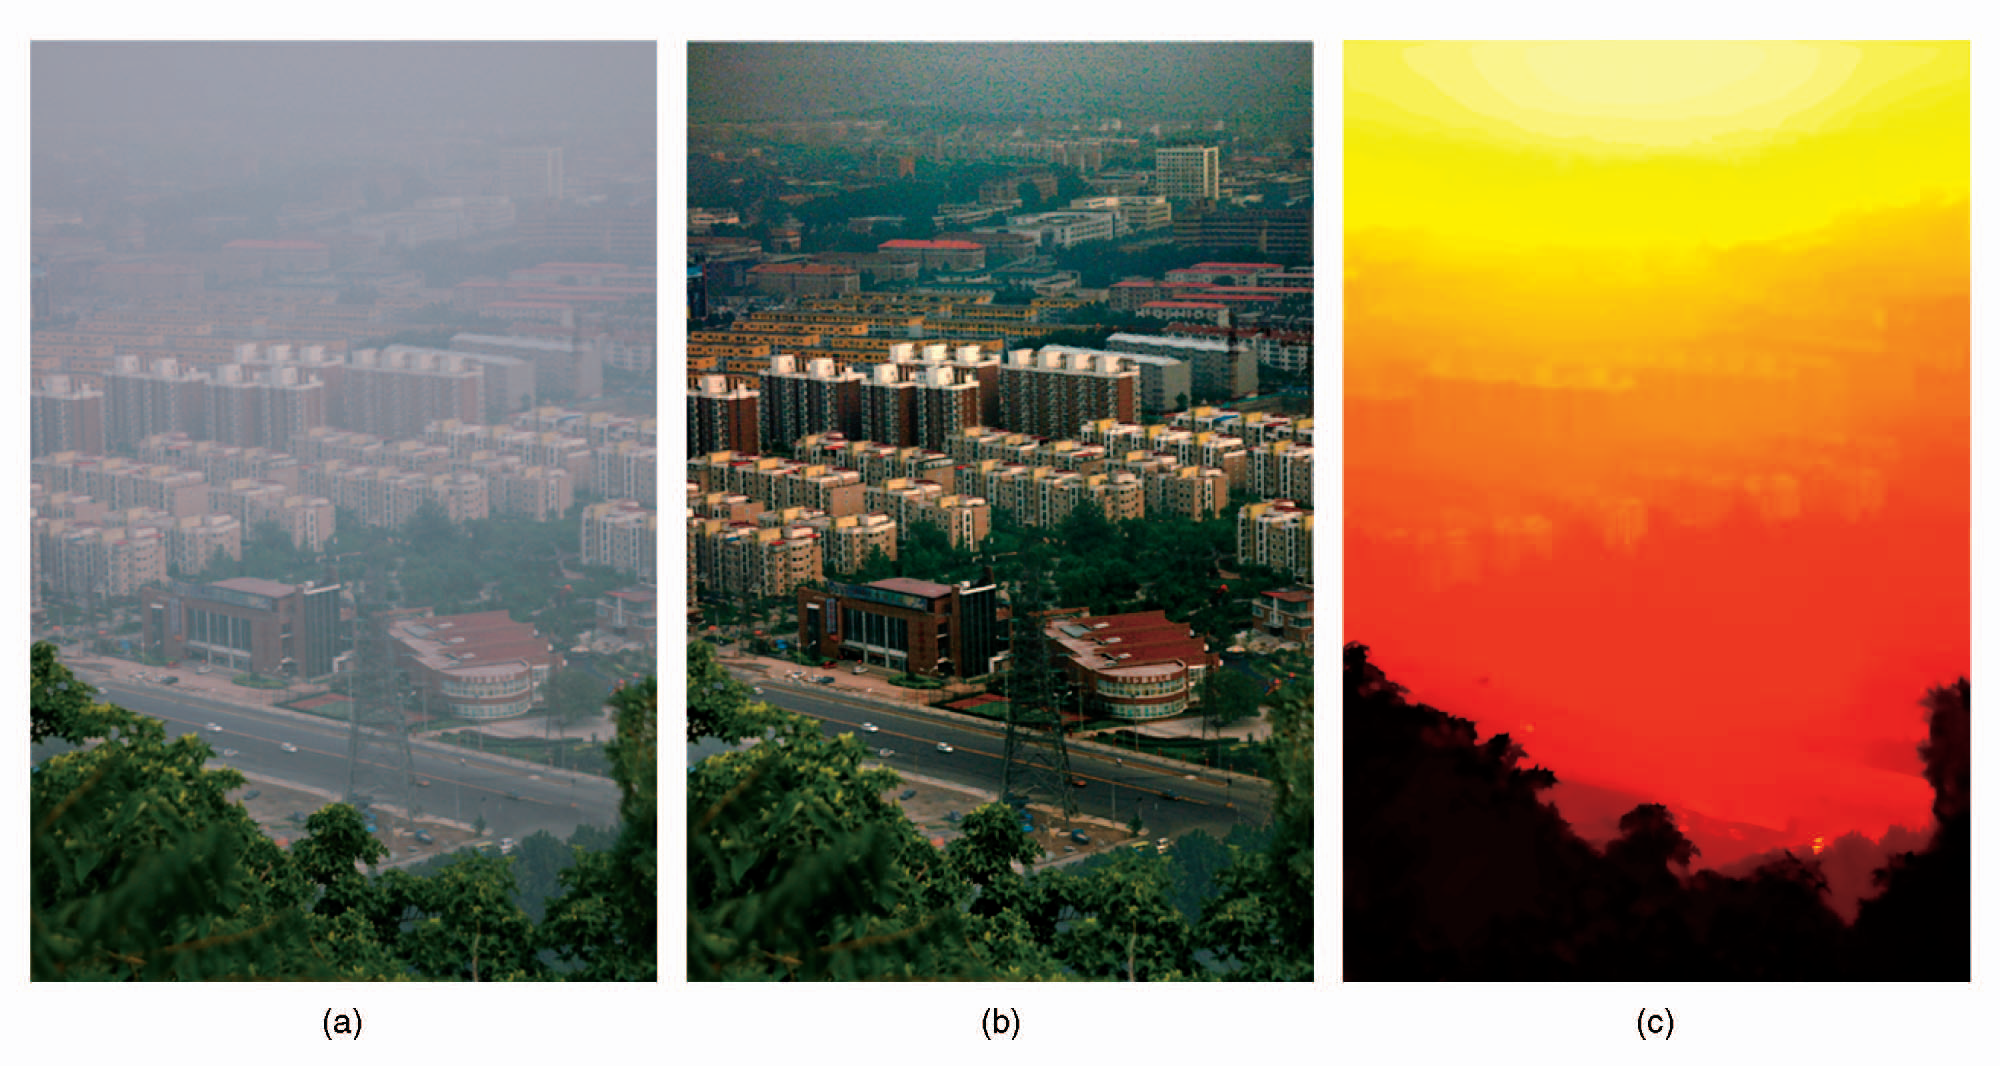
\includegraphics[width=\textwidth]{img/02.png}
    \caption{Haze removal using a single image. (a) Input hazy image. (b) Image after haze removal by our approach. (c) Our recovered depth map.}
    \label{fig:01}
\end{figure}


\bibliographystyle{unsrt}
\bibliography{refs}
\end{document}